\documentclass{article}

%%%%%%%%%%%%%%%%%%%%%%%%%%%%%%%%%%%%%%%%%
% Lachaise Assignment
% Structure Specification File
% Version 1.0 (26/6/2018)
%
% This template originates from:
% http://www.LaTeXTemplates.com
%
% Authors:
% Marion Lachaise & François Févotte
% Vel (vel@LaTeXTemplates.com)
%
% License:
% CC BY-NC-SA 3.0 (http://creativecommons.org/licenses/by-nc-sa/3.0/)
% 
%%%%%%%%%%%%%%%%%%%%%%%%%%%%%%%%%%%%%%%%%

%----------------------------------------------------------------------------------------
%	PACKAGES AND OTHER DOCUMENT CONFIGURATIONS
%----------------------------------------------------------------------------------------

\usepackage{amsmath,amsfonts,stmaryrd,amssymb} % Math packages

\usepackage{enumerate} % Custom item numbers for enumerations
\usepackage{listings}

\usepackage[ruled]{algorithm2e} % Algorithms

\usepackage[framemethod=tikz]{mdframed} % Allows defining custom boxed/framed environments

\usepackage{esvect}

\usepackage{listings} % File listings, with syntax highlighting
\usepackage{braket}
\usepackage{mathtools}

\lstset{
	basicstyle=\ttfamily, % Typeset listings in monospace font
}

%----------------------------------------------------------------------------------------
%	DOCUMENT MARGINS
%----------------------------------------------------------------------------------------

\usepackage{geometry} % Required for adjusting page dimensions and margins

\geometry{
	paper=a4paper, % Paper size, change to letterpaper for US letter size
	top=2.5cm, % Top margin
	bottom=3cm, % Bottom margin
	left=2.5cm, % Left margin
	right=2.5cm, % Right margin
	headheight=14pt, % Header height
	footskip=1.5cm, % Space from the bottom margin to the baseline of the footer
	headsep=1.2cm, % Space from the top margin to the baseline of the header
	%showframe, % Uncomment to show how the type block is set on the page
}

%----------------------------------------------------------------------------------------
%	FONTS
%----------------------------------------------------------------------------------------

\usepackage[utf8]{inputenc} % Required for inputting international characters
\usepackage[T1]{fontenc} % Output font encoding for international characters

\usepackage{XCharter} % Use the XCharter fonts

%----------------------------------------------------------------------------------------
%	COMMAND LINE ENVIRONMENT
%----------------------------------------------------------------------------------------

% Usage:
% \begin{commandline}
%	\begin{verbatim}
%		$ ls
%		
%		Applications	Desktop	...
%	\end{verbatim}
% \end{commandline}

\mdfdefinestyle{commandline}{
	leftmargin=10pt,
	rightmargin=10pt,
	innerleftmargin=15pt,
	middlelinecolor=black!50!white,
	middlelinewidth=2pt,
	frametitlerule=false,
	backgroundcolor=black!5!white,
	frametitle={Command Line},
	frametitlefont={\normalfont\sffamily\color{white}\hspace{-1em}},
	frametitlebackgroundcolor=black!50!white,
	nobreak,
}

% Define a custom environment for command-line snapshots
\newenvironment{commandline}{
	\medskip
	\begin{mdframed}[style=commandline]
}{
	\end{mdframed}
	\medskip
}

%----------------------------------------------------------------------------------------
%	FILE CONTENTS ENVIRONMENT
%----------------------------------------------------------------------------------------

% Usage:
% \begin{file}[optional filename, defaults to "File"]
%	File contents, for example, with a listings environment
% \end{file}

\mdfdefinestyle{file}{
	innertopmargin=1.6\baselineskip,
	innerbottommargin=0.8\baselineskip,
	topline=false, bottomline=false,
	leftline=false, rightline=false,
	leftmargin=2cm,
	rightmargin=2cm,
	singleextra={%
		\draw[fill=black!10!white](P)++(0,-1.2em)rectangle(P-|O);
		\node[anchor=north west]
		at(P-|O){\ttfamily\mdfilename};
		%
		\def\l{3em}
		\draw(O-|P)++(-\l,0)--++(\l,\l)--(P)--(P-|O)--(O)--cycle;
		\draw(O-|P)++(-\l,0)--++(0,\l)--++(\l,0);
	},
	nobreak,
}

% Define a custom environment for file contents
\newenvironment{file}[1][File]{ % Set the default filename to "File"
	\medskip
	\newcommand{\mdfilename}{#1}
	\begin{mdframed}[style=file]
}{
	\end{mdframed}
	\medskip
}

%----------------------------------------------------------------------------------------
%	NUMBERED QUESTIONS ENVIRONMENT
%----------------------------------------------------------------------------------------

% Usage:
% \begin{question}[optional title]
%	Question contents
% \end{question}

\mdfdefinestyle{question}{
	innertopmargin=1.2\baselineskip,
	innerbottommargin=0.8\baselineskip,
	roundcorner=5pt,
	nobreak,
	singleextra={%
		\draw(P-|O)node[xshift=1em,anchor=west,fill=white,draw,rounded corners=5pt]{%
		Question \theQuestion\questionTitle};
	},
}

\newcounter{Question} % Stores the current question number that gets iterated with each new question

% Define a custom environment for numbered questions
\newenvironment{question}[1][\unskip]{
	\bigskip
	\stepcounter{Question}
	\newcommand{\questionTitle}{~#1}
	\begin{mdframed}[style=question]
}{
	\end{mdframed}
	\medskip
}

%----------------------------------------------------------------------------------------
%	WARNING TEXT ENVIRONMENT
%----------------------------------------------------------------------------------------

% Usage:
% \begin{warn}[optional title, defaults to "Warning:"]
%	Contents
% \end{warn}

\mdfdefinestyle{warning}{
	topline=false, bottomline=false,
	leftline=false, rightline=false,
	nobreak,
	singleextra={%
		\draw(P-|O)++(-0.5em,0)node(tmp1){};
		\draw(P-|O)++(0.5em,0)node(tmp2){};
		\fill[black,rotate around={45:(P-|O)}](tmp1)rectangle(tmp2);
		\node at(P-|O){\color{white}\scriptsize\bf !};
		\draw[very thick](P-|O)++(0,-1em)--(O);%--(O-|P);
	}
}

% Define a custom environment for warning text
\newenvironment{warn}[1][Warning:]{ % Set the default warning to "Warning:"
	\medskip
	\begin{mdframed}[style=warning]
		\noindent{\textbf{#1}}
}{
	\end{mdframed}
}

%----------------------------------------------------------------------------------------
%	INFORMATION ENVIRONMENT
%----------------------------------------------------------------------------------------

% Usage:
% \begin{info}[optional title, defaults to "Info:"]
% 	contents
% 	\end{info}

\mdfdefinestyle{info}{%
	topline=false, bottomline=false,
	leftline=false, rightline=false,
	nobreak,
	singleextra={%
		\fill[black](P-|O)circle[radius=0.4em];
		\node at(P-|O){\color{white}\scriptsize\bf i};
		\draw[very thick](P-|O)++(0,-0.8em)--(O);%--(O-|P);
	}
}

% Define a custom environment for information
\newenvironment{info}[1][Info:]{ % Set the default title to "Info:"
	\medskip
	\begin{mdframed}[style=info]
		\noindent{\textbf{#1}}
}{
	\end{mdframed}
}
 

\title{CHEM 548 Project 1\\Finite Difference Method}

\author{Daniel McIntosh} 


\begin{document}
\maketitle

\section*{Code Description}
The purpose of this project was to implement the finite difference method for solving differential equations and applying them to the one-dimensional Schrodinger equation with various potentials. My implementation of this method can be found publicly available at:
 
 "$https://github.com/DanielMcIntoshK/CHEM548\_projects$" 
 
under the Project 1 folder. To compile the code simply use the following commands from the Project 1 directory:

\begin{lstlisting}
make
bin/Project1
\end{lstlisting}

Building this project should be possible on any computer that contains a c++ compiler as no libraries were used in this project except those found in the c++ standard template library.

It will generate the files "PIB", "FIN", "PBRect", "Harm", "Morse1", and "Morse2" in the Outputs directory (which has already been generated on the github). These files are the results of the particle in a box, finite well, rectangular barrier, harmonic, and Morse computations respectively. These files contain space delineated data. The first row is the eigenvalues of the computed states. The rest of the file is a matrix where the columns are the eigenvectors representing the wavefunctions of the associated eigenvalues.

Additionally there is a folder called "reader" which contains a python program that can open these files and graph the first $n$ wavefunctions on top of the potential, as well as preform some other tasks such as computing Frank Condon factors and integrals.

Diagonalization of the matrices was accomplished using a hermitian Jacobian rotation algorithm. This method works by constructing unitary rotational matricies to rotate away the largest values within the upper-triangle of a matrix. The eigenvalues are the diagonal elements once all values above a threshold have been removed from the off diagonal elements, and the eigenvectors are the product of all the rotational matricies.

\section*{Results}

Each of the computations were preformed using a grid of 100 points, and a mass of 1.

\newpage
\subsection*{Particle in a Box}

The computation was run for a potential that was zero within some dimensions and infinity outside of them. The calculated eigenvalues can be found in Table \ref{tab:pib}, and the wavefunctions in Figure \ref{fig:pib}. 

The generated eigenvalues were close to the theoretical exact values ($E_n=\frac{n^2\pi^2}{2mL^2}$), and the wavefunctions had the correct form of a sin wave with an increasing number of nodes that terminates at the barrier.

\begin{figure}[h]
\centering
	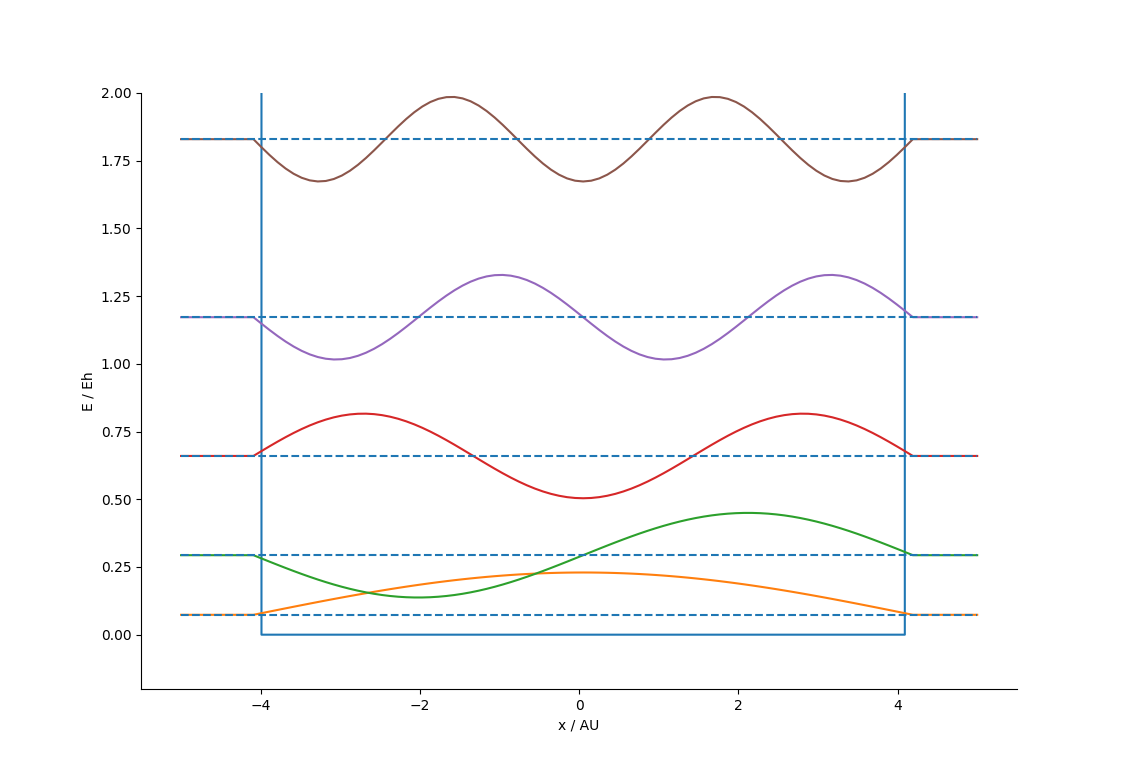
\includegraphics[width=.75\linewidth]{images/pib.png}
	\caption{The Wavefunctions of the Particle in a Box}
	\label{fig:pib}
\end{figure}

\begin{table}[h]
\centering
\begin{tabular}{ |c|c|c|}
\hline
n & exact & computed \\
\hline
1 & 0.0771063 & 0.0733801 \\
2 & 0.308425 & 0.293413 \\
3 & 0.693957 & 0.659775\\
4 & 1.23370 & 1.17193\\
5 & 1.92766 & 1.82912\\
6 & 2.77583 & 2.63039\\
\hline
\end{tabular}
\caption{Computed energies of the particle in a box with a length of 8 compared to the exact values}
\label{tab:pib}
\end{table}

\newpage
\subsection*{Finite Well}
The Finite well computations were the same as the particle in a box except the boundry was lowered to be a finite height instead of infinite. The wavefunctions can be be seen in Figure \ref{fig:fin}. The probability of finding the particle outside of the well was calculated using a number of well depths Table \ref{tab:fin}.

The probability of finding the particle decreased as the well depth increased which is what we would expect. Also the wave functions have the correct form, looking the same as the previous section except stretching out more and permeating into the boundry.

\begin{figure}[h]
\centering
	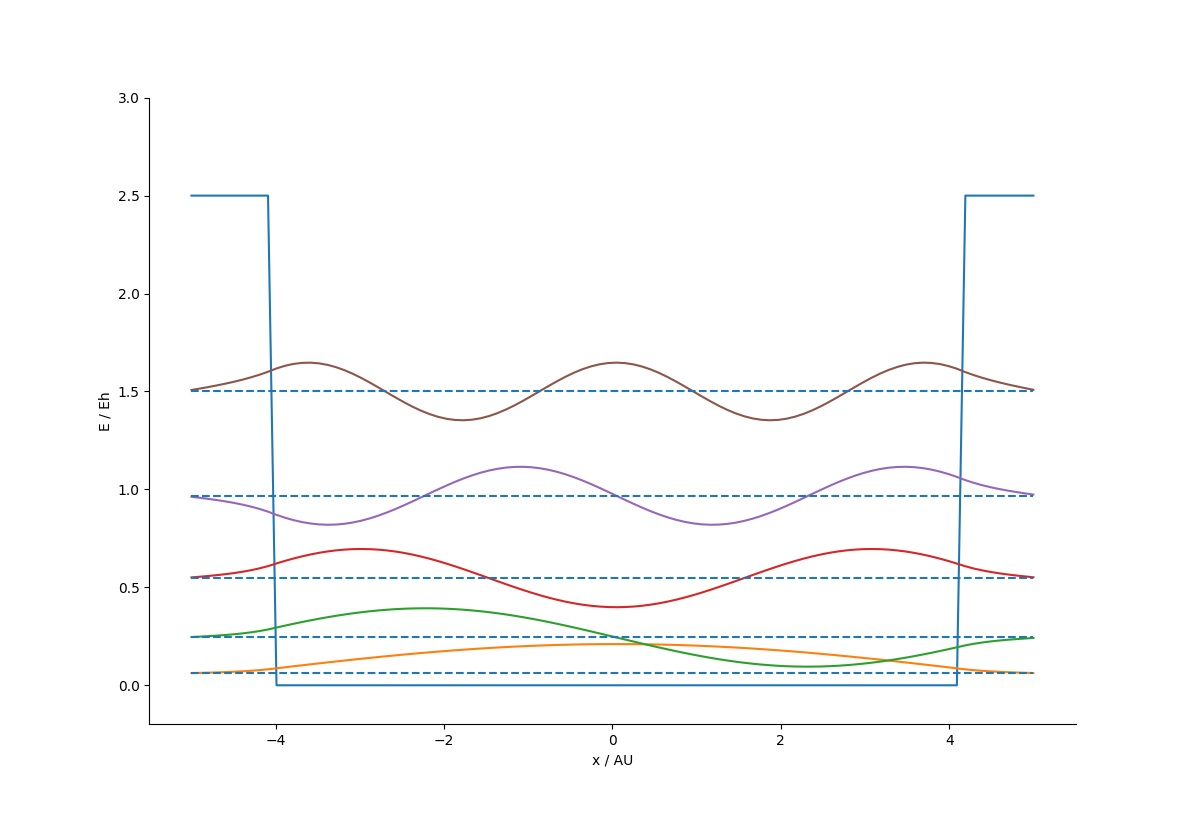
\includegraphics[width=.75\linewidth]{images/finite.png}
	\caption{The Wavefunctions of the Finite well with a well depth of 2.5 Eh }
	\label{fig:fin}
\end{figure}

\begin{table}[h]
\centering
\begin{tabular}{ |c|c|}
\hline
Well Depth (Eh) & Prob\\
\hline
0.2 & 0.057055\\
0.4 & 0.037867 \\
0.6 & 0.027045 \\
0.8 & 0.020402\\
1.0 & 0.016037\\
\hline
\end{tabular}
\caption{The probability of finding the particle outside of the well for the lowest energy wavefunction for various well depths}
\label{tab:fin}
\end{table}   

\newpage
\subsection*{Rectangular Barrier}
The rectangular barrier was placed in the middle of the particle in a box problem. Two different options were tried, one with a narrow barrier (Figure \ref{fig:narbar}) and one with a wide barrier (Figure \ref{fig:widebar}). 

The wide barrier showed two distinct near degenerate orthogonal states for each energy level. However the narrow barrier showed the states become more overlapping and energy splitting occurring between the previously degenerate states.

\begin{figure}[h]
\centering
	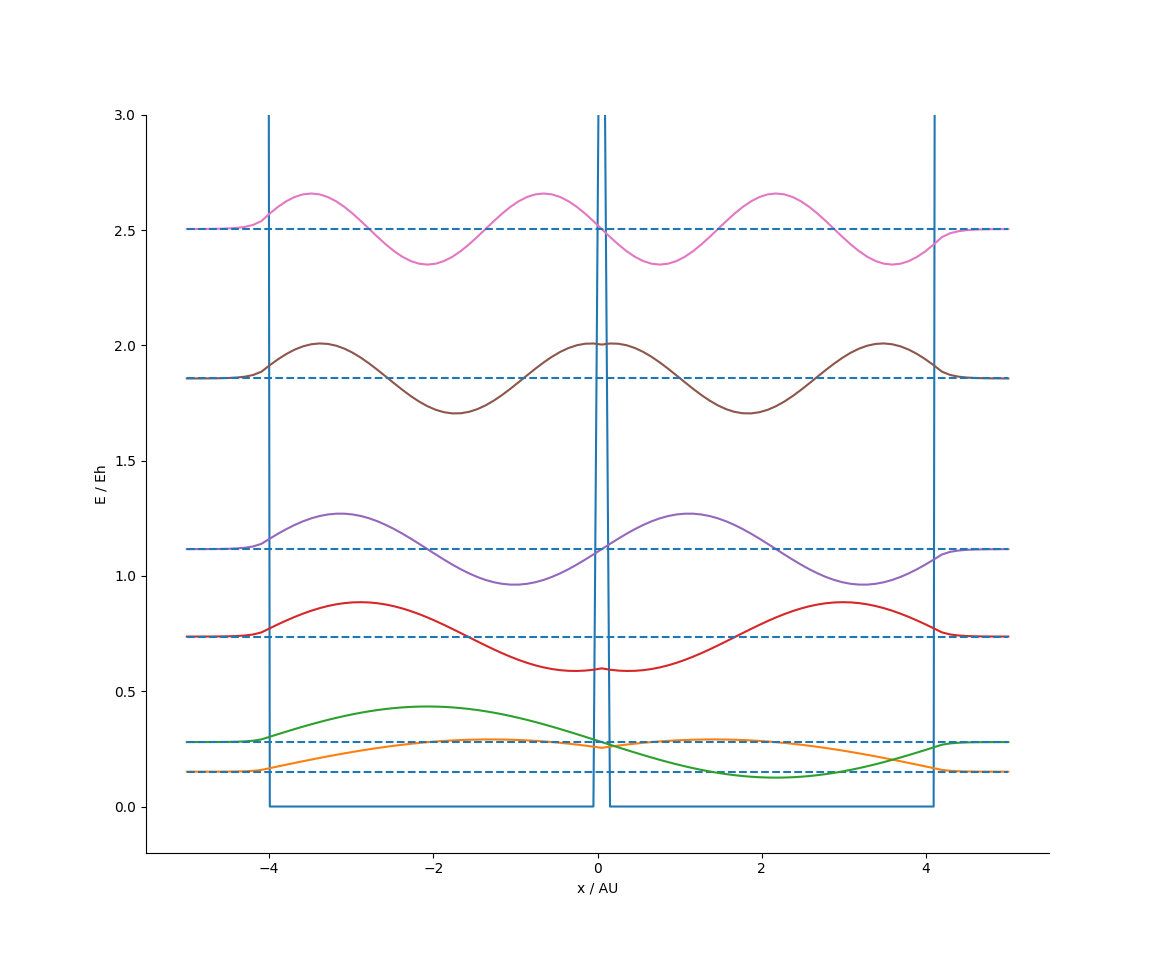
\includegraphics[width=.6\linewidth]{images/rectnarrow.png}
	\caption{The Wavefunctions of particle in a box with a narrow rectangular barrier }
	\label{fig:narbar}
\end{figure}

\begin{figure}[h]
\centering
	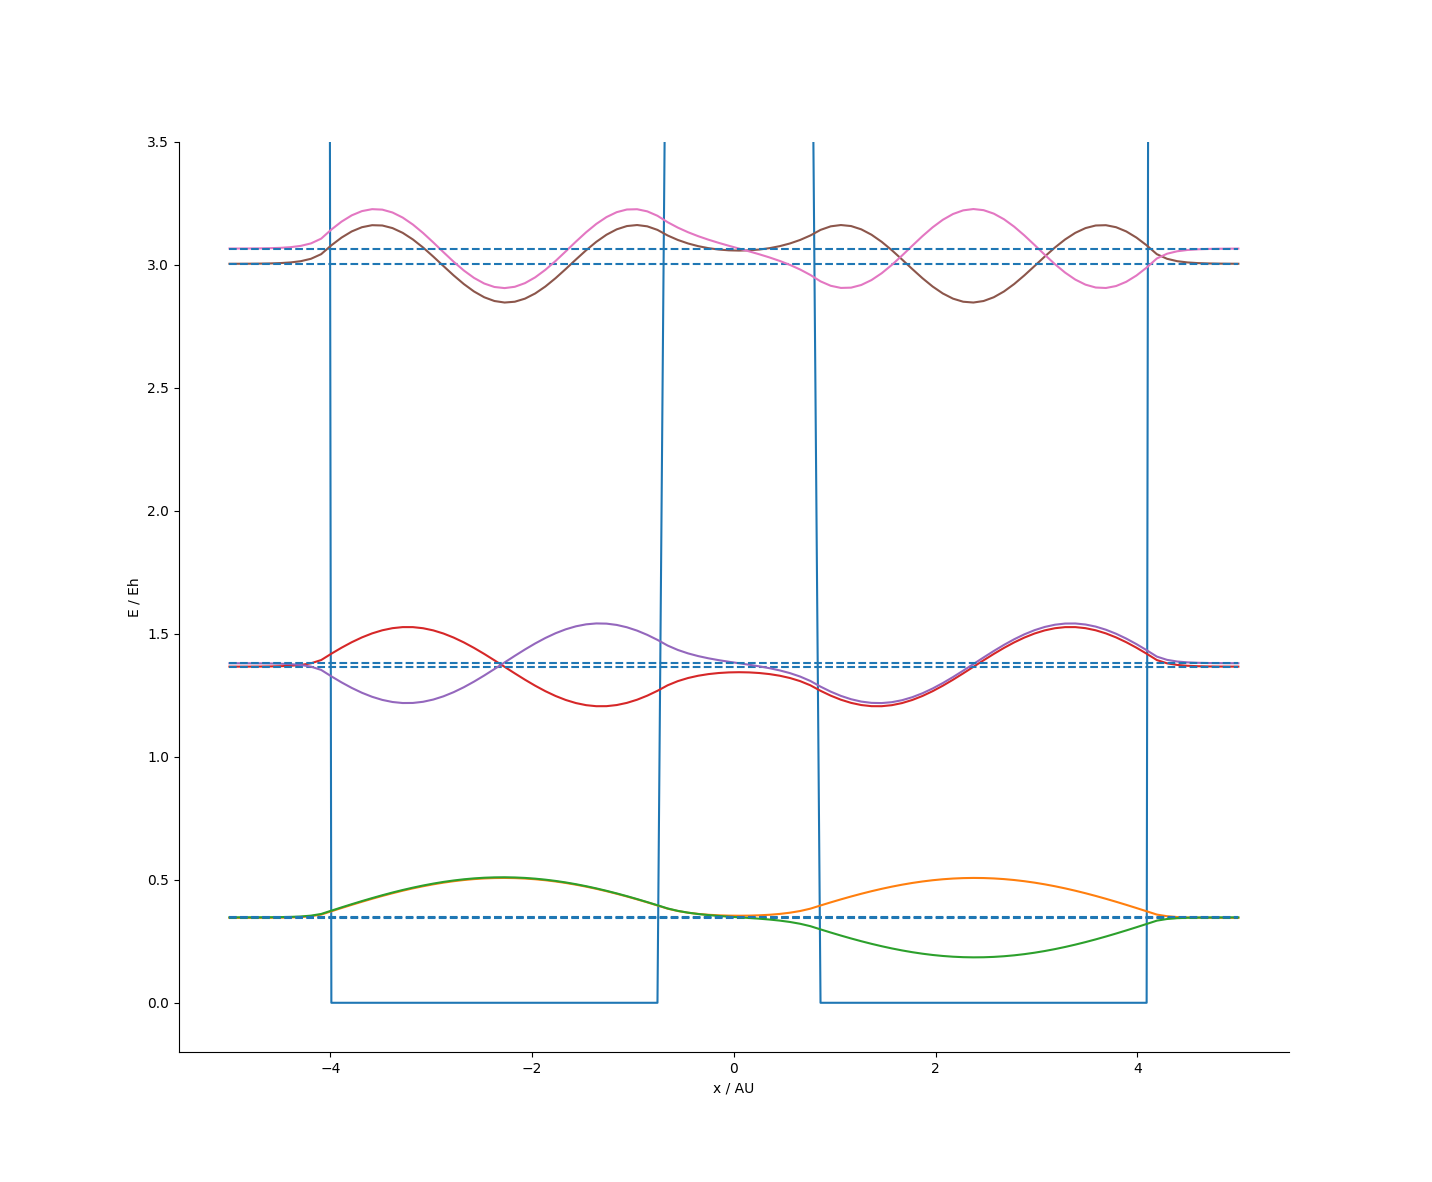
\includegraphics[width=.6\linewidth]{images/rectwide.png}
	\caption{The Wavefunctions of particle in a box with a wide rectangular barrier  }
	\label{fig:widebar}
\end{figure}

\newpage
\subsection*{Harmonic}
A harmonic potential was used with a k value of 1. The calculated eigenvalues are shown next to the expected exact amount in Table \ref{tab:harm}. The wavefunctions can be found in Figure \ref{fig:harm}.

The energy results and wavefunctions are in agreement with what we would expect from the harmonic oscillator.

\begin{table}[h]
\centering
\begin{tabular}{ |c|c|c|}
\hline
n & exact (Eh) & computed (Eh) \\
\hline
0 & 0.5& 0.499687\\
1 & 1.5& 1.49844 \\
2 & 2.5& 2.49593 \\
3 & 3.5& 3.49217 \\
4 & 4.5& 4.48716 \\
5 & 5.5& 5.48094 \\
\hline
\end{tabular}
\caption{The energies of the harmonic oscillator compared to the exact values}
\label{tab:harm}
\end{table}

\begin{figure}[h]
\centering
	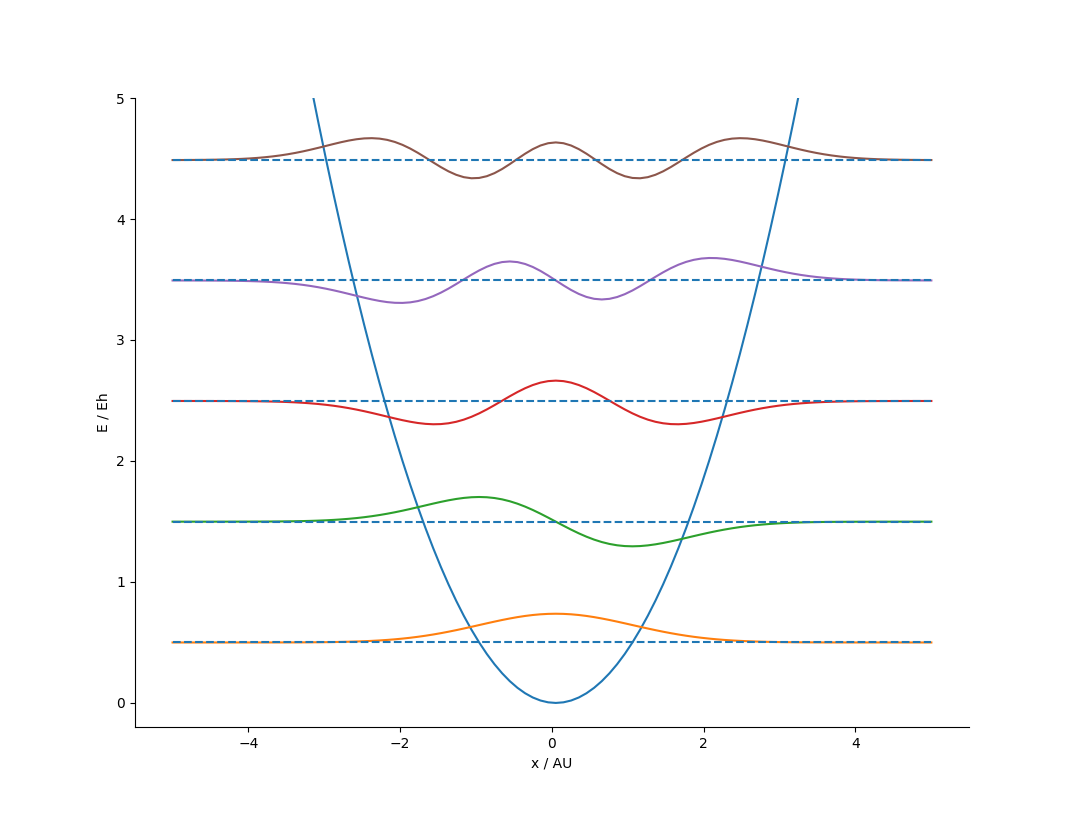
\includegraphics[width=.75\linewidth]{images/harm.png}
	\caption{The Wavefunctions of harmonic oscillator  }
	\label{fig:harm}
\end{figure}

\newpage
\subsection*{Morse}
Two Morse potentials were created, the first one with an dissociation energy of 5.0 Eh, and an exponent of 2.0. The second Morse potential and a dissociation energy of 3.0 Eh and an exponent of .5. The second Morse potential was displaced from the first up by 7.0 and over by 1.5. A figure of the potentials and their wavefunctions can be found in Figure \ref{fig:morse}.
 
The Frank Condon factors were computed from the overlap of the wavefunctions Table \ref{tab:morse}. From these a simulated electronic spectra was generated where it was assumed that it was a temperature such that the lowest energy is 90$\%$ thermally occupied and the next level is 10$\%$ (Figure \ref{fig:spectra}).

\begin{figure}[h]
\centering
	\includegraphics[width=.75\linewidth]{images/morse.png}
	\caption{The Wavefunctions of two morse potentials and their wavefunctions  }
	\label{fig:morse}
\end{figure}
\begin{table}[h]
\centering
\begin{tabular}{ |c|c|c|}
\hline
         & $\bra{\Phi_0^0}$ & $\bra{\Phi_1^0}$\\
\hline
$\ket{\Phi_0^1}$ & 0.1532           & 0.5806 \\
$\ket{\Phi_1^1}$ & 0.2271           & 0.4376 \\
$\ket{\Phi_2^1}$ & 0.2697           & 0.3127 \\
$\ket{\Phi_3^1}$ & 0.3173           & 0.2054 \\
$\ket{\Phi_4^1}$ & 0.3746           & 0.0841 \\
$\ket{\Phi_5^1}$ & 0.4109           & 0.0599 \\
$\ket{\Phi_6^1}$ & 0.4101           & 0.1922 \\
$\ket{\Phi_7^1}$ & 0.3679           & 0.2789 \\
\hline
\end{tabular}
\caption{The Frank Condon factors computed from the first two states of the lower Morse potential and the first 8 states of the upper Morse potential}
\label{tab:morse}
\end{table}
\begin{figure}[h]
\centering
	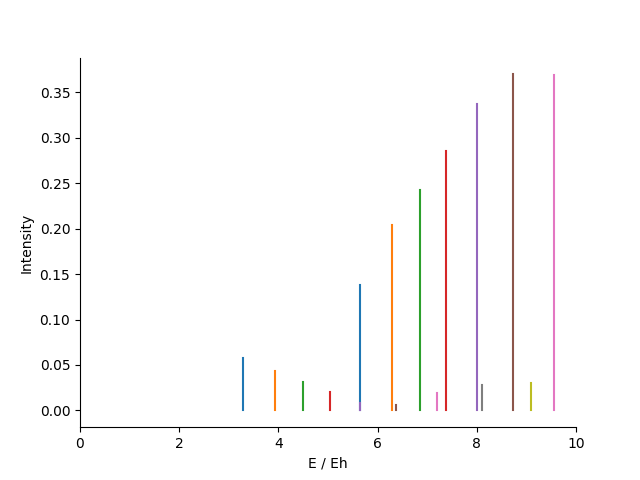
\includegraphics[width=.75\linewidth]{images/simulate.png}
	\caption{A simulated electronic spectra }
	\label{fig:spectra}
\end{figure}

\newpage
\section*{Conclusion}
Presented here were a number of systems modeled with the finite difference method. For each one we were able to find numerical values for energy that closely matched theoretical values, as well as generate wavefunctions that were qualitatively correct. This despite the simplicity of the approximation taken.


However it should be noted that the accuracy shown here was only attainable due to the fact that we have only modeled 1D systems. Any attempt to use this method on even 2D or 3D systems would quickly become unfeasible. 

\end{document}
